\documentclass{article}
\usepackage{../fasy-hw}
\usepackage{centernot}
\usepackage{amssymb}
\usepackage{enumitem}


%% UPDATE these variables:
\renewcommand{\hwnum}{2}
\title{Discrete Structures, Homework 1}
\author{Braeden Hunt (Tinnittin)}
\collab{n/a}
\date{due: 5 February 2021}

\begin{document}

\maketitle

This homework assignment should be
submitted as a single PDF file both to D2L and to Gradescope.

General homework expectations:
\begin{itemize}
    \item Homework should be typeset using LaTex.
    \item Answers should be in complete sentences and proofread.
    \item You will not plagiarize.  \item List collaborators at the start of each question using the \texttt{collab} command.
    \item Put your answers where the \texttt{todo} command currently is (and
        remove the \texttt{todo}, but not the word \texttt{Answer}).
\end{itemize}

% ============================================
% ============================================
\collab{n/a} \nextprob{Everyday Mathematical Arguments}
% ============================================
% ============================================
Your sister and you decided to partner on a car washing endeavor, where you
charge cars $\$10$ for a car wash and to split the earnings.  Since you are
doing this at your parents house and they had extra soap, sponges, and a hose
available, there are no costs to you.  At the end of the first day, you have
earned $\$45$ and she had only earned $\$10$. She claimed that you did not pay
her the full payment she deserved. Her argument was: ``If we wash a car, you
earn $\$5$ and I earn $\$5$.  If you earned $\$45$, then we washed nine cars.  If
we wash nine cars, I have earned $\$45$.  I have earned $\$10$; therefore, you
did not give me all of the money that I earned.''  Now, she has not yet taken
Prof.~Fasy's Discrete Structures class, so she does not see the fallacy in her
argument. First, explain which statement that she made that she could not
correctly conclude and explain why.  Second, counter her argument, using
everyday English. The last sentence of your argument should be ``Therefore, I
earned $\$45$ and you earned $\$10$. Third, write this counter argument using
logic statements by first listing the logic statements then writing the argument
mathematically.  Be sure to explain which arguments from Table 2.3.1 that you
are using.

\paragraph{Answer}

She made the converse error. The statement ``if we wash a car, we both earn $\$5$ each" is true.
However, the converse statement ``if I earned $\$45$, then I washed nine cars" is not true because the statement is conditional, not biconditional. I could have earned money by doing other things such as vacuuming cars.
Therefore, I earned $\$45$ and you earned $\$10$.

Consider the following statements:
\begin{enumerate}
    \item p = ``We wash a car''
    \item q = ``I get $\$5$''
    \item r = ``you get $\$5$''
\end{enumerate}
$p \implies q$

$p \implies r$

$p \centernot \iff q$

$\therefore q \centernot \implies p$

$\therefore q \centernot \implies r$

This means that it is possible for me to earn $\$45$ while my sister only earned $\$10$.


% ============================================
% ============================================
\collab{n/a}
\nextprob{Existential Statements}
% ============================================
% ============================================

Are the following statements true or not true?    Prove or disprove.

\begin{enumerate}

    \item All even integers are equal to an odd integer plus one.

        \paragraph{Answer}

	If an integer is even, then it is equal to an odd integer plus one.

	All even integers $i$ can be written in the form $i=2k$ such that $k \in \Z$,
	and all odd integers $n$ can be written in the form $n=2k-1$ such that $k \in \Z$ .
	Therefore, we can see that $n=i-1$ or $n+1=i$. This shows that all integers can 
	be written as one more than an odd number.

    \item All horses are the same color.

        \paragraph{Answer}
	
	If something is a horse, than it is the same color as all other horses.

	The negation of this is that there exists a horse that is a different color 
	than some other horse. This negation is false because there are horses brown 
	horses and black horses, as well as many other colors. As the negation of the
	statement is false, the statement is true.

\end{enumerate}


% ============================================
% ============================================
\collab{n/a}
\nextprob{Division into Cases}
% ============================================
% ============================================

When working at Lockheed Martin, I was invited to play Texas
Hold'em\footnote{For rules, see
here:\url{https://www.pokernews.com/poker-rules/texas-holdem.htm}} at my
colleague's house.  I play with the following rules:
\begin{itemize}
    \item Never fold before the flop.
    \item Never increase the bet.
    \item If it is possible that my hand is \emph{three of a kind} or better,
        match the bet.  Otherwise, fold.
\end{itemize}
My current hand is the jack of hearts and the 10 of diamonds, and the flop is 10
of hearts, 3 of clubs, and king of hearts.

\begin{enumerate}

    \item What are the cases that could occur for the Turn card?  What is the
        outcome (match or fold) for these different cases? (Note: rather than
        listing every possible card, try to categorize the cards into as few
        classes as possible).

    \paragraph{Answer} Note: I am not familiar with this game at all. After reading the rules, I believe these are the following are the only ways to get a 3 of a Kind or better with the given hands.

	Matching Case:
	\begin{itemize}

    	\item 3 of a Kind: The next card is a 10. 
\end{itemize}
Folding Case:
	\begin{itemize}

    	\item Any card that is not a 10. 
\end{itemize}
    \item Suppose that the Turn card is the jack of clubs.
        What are the cases that could occur for the River card, and what is the
        outcome (match or fold) for these different cases?  (Again, try to
        describe this in as few cases as possible).

    \paragraph{Answer}
    Matching Case:
	\begin{itemize}

    	\item Full House: The next card is a 10 or a jack. 
	
\end{itemize}
Folding Case:
	\begin{itemize}

    	\item Any card that is not a 10 or a jack. 
\end{itemize}

\end{enumerate}


% ============================================
% ============================================
\collab{n/a}
\nextprob{Bipartite Graphs}
% ============================================
% ============================================

Exercise Set 4.9, Question 23.

\paragraph{Answer}
\begin{enumerate}[label=\Alph*]
\item See Figure \ref{Graph1}
\item See Figure \ref{Graph2}
\item See Figure \ref{Graph3}
\item $n$ vertices have $m$ degree and $m$ vertices have $n$ degree.
\item The total degree of the graph is equal to $2*m*n$.
\item The total number of edges is equal to $m*n$ because there are m vertices that are each have n degree.
\end{enumerate}


% ============================================
% ============================================
\collab{n/a}
\nextprob{Four Color Theorem}
% ============================================
% ============================================
Read Chapter 1 of \emph{Four Colors Suffice} and answer the following questions:

\begin{enumerate}

    \item Consider the map of the continental US on Page 5.  Why can we color
        Utah and New Mexico the same color, even though the two states touch at
        a point?

        \paragraph{Answer}
       	They don't share a boundary line, just a meeting point. If we required maps 
		to be colored such that any two countries that shared just a meeting point 
		where different colors, the solution to the four color problem would be infinite,
		as you could make a pie shaped graph with infinite slices.

    \item Again, looking at the map of the continental US on Page 5, explain why
        Michigan does not satisfy the conditions for the four color theorem.

        \paragraph{Answer}
        	One of the conditions for the four color theorem is that each region be connected 
		to itself. Michigan is spit into two parts, so it does not satisfy this condition.

    \item Explain why we an omit the states of Hawaii and Alaska in order to
        construct a four-coloring of the states in the USA.

        \paragraph{Answer}
        Since they share no boundaries with any other state (region), they do not affect the coloring at all.

    \item Is the following statement TRUE or FALSE?  Explain. Four colors are
        necessary to color all maps.

        \paragraph{Answer}
        False, there are maps that you can color in one, two, and three colors.

    \item Explain one application of the four color theorem that does not
        involve coloring geographic maps.

        \paragraph{Answer}
        Mobile phone towers often overlap areas of coverage. However, they 
	cannot transmit on the same frequency, or else they will have issues with the signal. 
	The four color theorem states that these networks of towers can use just four 
	frequencies to avoid the issue.

    \item (Extra Credit). Provide a four-coloring of the McGregor April Fool's
        Hoax on Page 11.

 	\paragraph{Answer} See Figure \ref{bonus}.


% ============================================
% ============================================
\collab{n/a}
\nextprob{Fred Brooks}
% ============================================
% ============================================


Write a short (1-2 paragraph) biography of Fred Brooks.  He wrote the book
entitled \emph{The Mythical Man Month}~\cite{brooks-manmonth}.  In your
biography, explain what the title of this book means.
\textbf{In your own words}, describe who they are and why they are important in
the history of computer science.  If you use external resources, please provide
proper citations. If you do not use external sources, please write ``I did not
use any sources to write this biography'' as the last sentence of the
biography.

\paragraph{Answer}

Fred Brooks is a American computer scientist . He received a bachelores degree
 in physics and a doctorate in applied mathematics. He later worked for IMB 
creating computers and software. While there, he defined the byte, invented 
computer interrupts, and managed the team that wrote the IBM operating system. 

These are all incredible accomplishments, but his work in software engineering
 management was equally if not more important. In his book \emph{The Mythical Man Month}, 
Brooks discusses his thoughts on this process. One of the biggest is the idea that you can't throw
more man power at a behind schedule software project as it will actually make delay the project slower.
This is in opposition of the "Man Month," a unit of work that one person can do in one month. If a project
will take 6 man months to complete, it supposedly would take one person 6 months to do, or 6 people one
to do. However, due to the complex and intertwined nature of software projects, adding more people
on a delayed project will delay it further, because the original developers will have to slow down 
and catch the new developers up to speed, and as tasks are divided further among people, the
amount of avenues of communication increase, leading to inefficient methods of asking questions
and getting ideas across. 

Sources:
Paragraph 1: https://www.britannica.com/biography/Fred-Brooks

Paragraph 2: I did not use any sources to write this paragraph. I've learned about this through coworkers in the past.

%% ... the bibliography
\newpage
\bibliographystyle{acm}
\bibliography{biblio}


\pagebreak
\begin{figure}
\caption{$K_{4, 2}$}
\centering
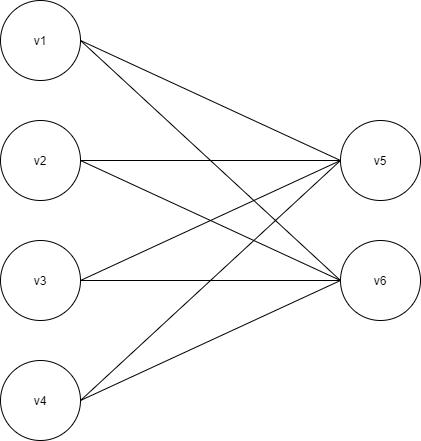
\includegraphics[width=0.5\textwidth]{Graph1}
\label{Graph1}
\end{figure}

\begin{figure}
\caption{$K_{1, 3}$}
\centering
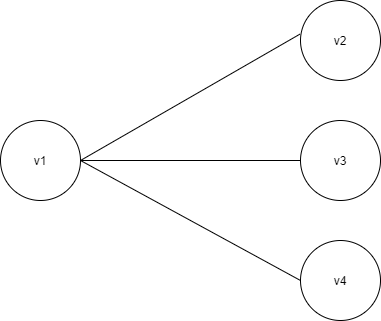
\includegraphics[width=0.5\textwidth]{Graph2}
\label{Graph2}
\end{figure}

\begin{figure}
\caption{$K_{3, 4}$}
\centering
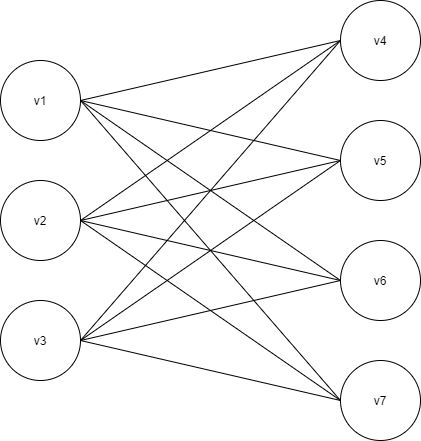
\includegraphics[width=0.5\textwidth]{Graph3}
\label{Graph3}
\end{figure}

\begin{figure}
\caption{McGregor April Fool's}
\centering
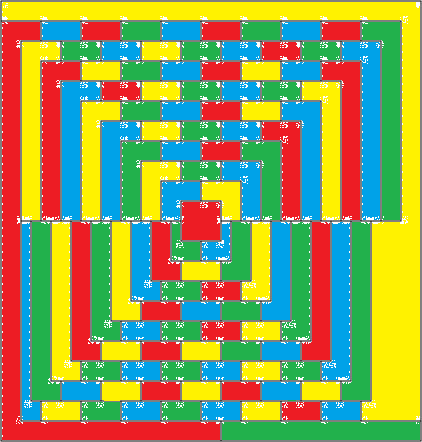
\includegraphics[width=0.5\textwidth]{bonus}
\label{bonus}
\end{figure}

\end{enumerate}
\end{document}

